\appendix
\newpage
\section{OAPs focal lengths relations}\label{sec:EFL2PFL}
This section describe the relation between the parental and the effective focal length for an off-axis parabola. The sketch figure~\ref{fig:EFL2PFL_sketch} describes the situation with :
\begin{itemize}
	\item EFL the effective focal length
	\item PFL the parental focal length
	\item ($x_S, y_S$) the coordinate of the ray intersection with the parabola
	\item the parabola of equation \begin{equation}
	y = \frac{x^2}{4\text{PFL}}-\text{PFL}	\label{eq:parabola_general}
\end{equation}	 
\end{itemize}

\begin{figure}[H]
	\begin{center}
		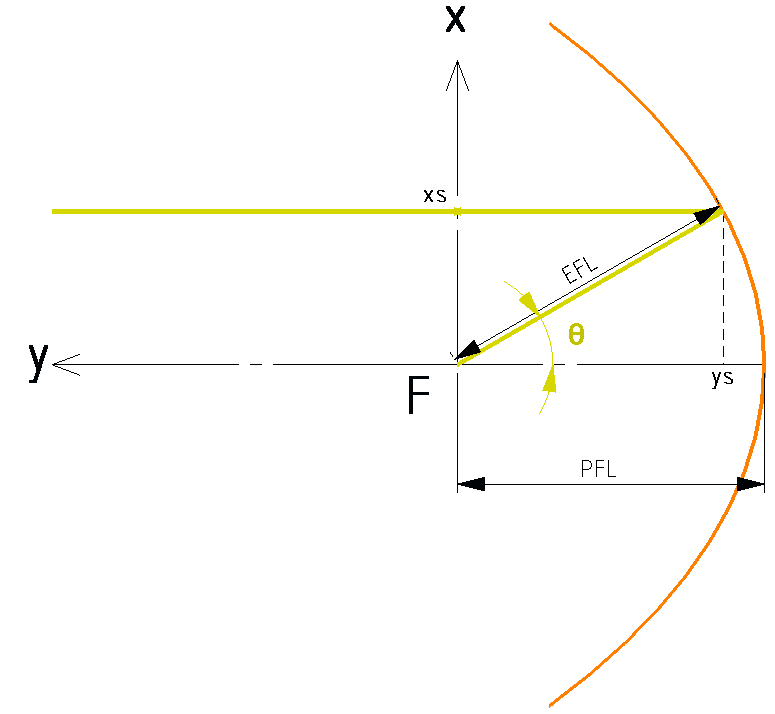
\includegraphics[width=0.5\textwidth]{images/EFL2PFL_sketch.PNG}
		\caption{Sketch of a ray reflected on an OAP}\label{fig:EFL2PFL_sketch}
	\end{center}
\end{figure}
The relation between EFL and PFL can be determined with the following set of equations.
\begin{eqnarray}
	x_S &= &\text{EFL}\sin\theta \nonumber\\
	y_S &= &\text{EFL}\cos\theta \label{eq:xs_ys}
\end{eqnarray}

Using \eqref{eq:parabola_general} and \eqref{eq:xs_ys} we have~:
\begin{eqnarray}
	4\text{PFL}\left(y_S+\text{PFL}\right) &= &x_S^2 \nonumber \\
	4\text{PFL}\left(\text{EFL}\cos\theta+\text{PFL}\right) &= &\left(\text{EFL}\sin\theta\right)^2\nonumber\\ 
	4\text{PFL}^2 - 4\text{PFL}\,\text{EFL}\cos\theta-\text{EFL}^2\sin^2\theta &= &0 \nonumber
\end{eqnarray}
\begin{eqnarray}
	\text{PFL}_{1,2} &= &\frac{4\text{EFL}\cos\theta\pm\sqrt{\left(-4\text{EFL}\cos\theta\right)^2+16\text{EFL}^2\sin^2\theta}}{2*4}  \nonumber\\
	&= &\frac{1}{2}\left[\text{EFL}\cos\theta\pm\sqrt{\text{EFL}^2\cos^2\theta+\text{EFL}^2\sin^2\theta}\right] \nonumber
\end{eqnarray}
The final equation is :
\begin{equation}
	2\text{PFL} = \text{EFL}\left(1+\cos\theta\right)\label{eq:EFL2PFL}
\end{equation}






%\newpage
%\section{Focal length of the relay lens between the pyramid and the CCD}\label{sec:PYR2CCD}
%Gauss :
%\begin{eqnarray}
%	\frac{1}{p_i}-\frac{1}{p_o} &= &\frac{1}{f_{LR}}	\nonumber\\
%	1-\frac{f_{LR}}{p_i} &= &-\frac{f_{LR}}{p_o}\label{eq:gaussPyr}
%\end{eqnarray}
%Thales :
%\begin{eqnarray}
%	\frac{\diameter_\text{CCD}}{\diameter_\text{L}} &= &\frac{|p_i|-|f_{LR}|}{|p_i|}\nonumber\\
%	\frac{\diameter_\text{CCD}}{\diameter_\text{L}} &= &1-\frac{f_{LR}}{p_i}\label{eq:ThalesPyr}
%\end{eqnarray}
%Mixing~\eqref{eq:gaussPyr} and \eqref{eq:ThalesPyr} :
%\begin{equation}
%	\frac{\diameter_\text{CCD}}{\diameter_\text{L}} = \frac{f_{LR}}{p_o}\label{eq:ThalGaussPyr}
%\end{equation}
%In another hand :
%\begin{equation}
%	\text{F}\# = \frac{f_\text{OAP3}}{\diameter_\text{TT}} = \frac{p_o}{\diameter_L}\label{eq:FnumPyr}
%\end{equation}
%Mixing \eqref{eq:ThalGaussPyr} and \eqref{eq:FnumPyr} :
%\begin{equation}
%f_\text{LR} = \text{F}\#\,\,\diameter_\text{CCD}
%\end{equation}



\newpage
\section{ADC design}\label{app:ADC}
\subsection{Scope}
The previous report explains the different possibilities to configure an ADC. Here we are presenting the design we are going to implement for the case of the DAG telescope AO. This ADC will be for visible wavelength. The range is limited by the camera Nuvu spectral range and the star spectrum studied. We are taking only the Nuvu camera bandwidth into account for a first iteration (500~nm to 900~nm).\\

\subsection{Amici principle}
As said in the previous report, the Amici prisms are commonly used in the ADC systems. The ADCs are composed by a 2-doublet design which mixes two Amici prisms. This kind of prism is an alliance of two pieces of glass which have different dispersion (different refractive indexes). The materials must have the same refractive number for a mean wavelength so that at this frequency the incident and emergent rays are parallel (zero-deviation at $\lambda_{av}$). The two prisms can be rotated around the optical axis in order to change the dispersion and compensate it for each zenith angle. When the angle between them is 180° the dispersion is reduced at its minimum.

\begin{figure}[H]
\centering
	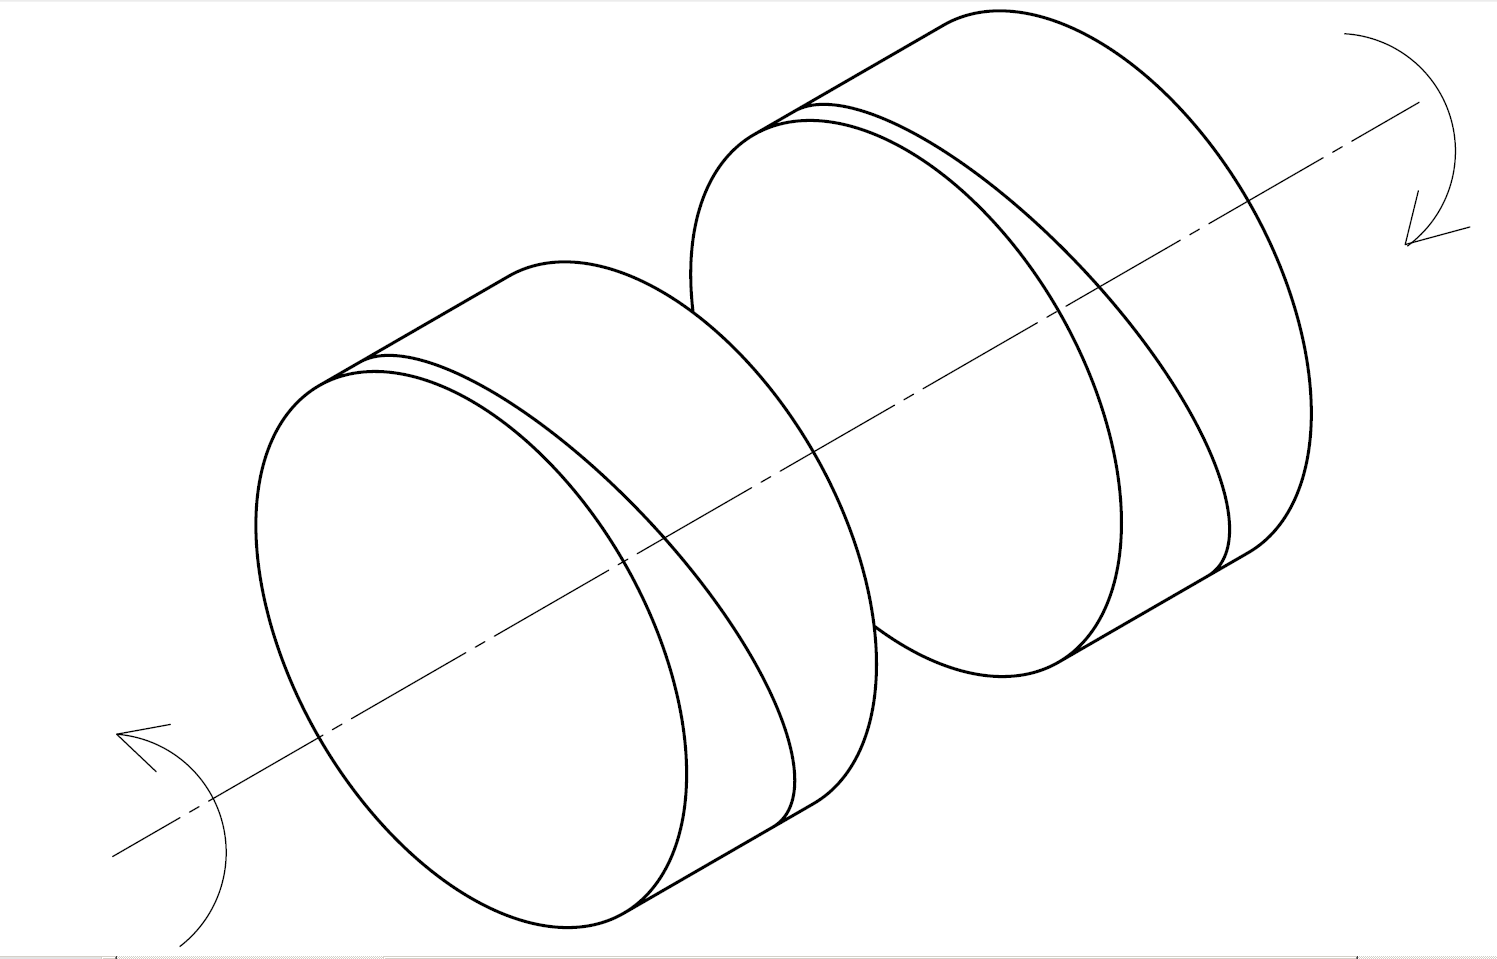
\includegraphics[width = 0.4\textwidth]{images/amiciISO.png}
	\caption{2-doublet Amici prisms design}
	\centering
\end{figure}



Another design can be a three-glass Amici prisms, which is called triplet-design. It consists of the insertion of a anomalous dispersion glass between the two firstly introduced surfaces. According to Kopon thesis\cite{KCG}, the doublet corrects only the first order of chromatism while the triplet acts on both primary and secondary chromaticism aberration.
\begin{figure}[H]
\centering
	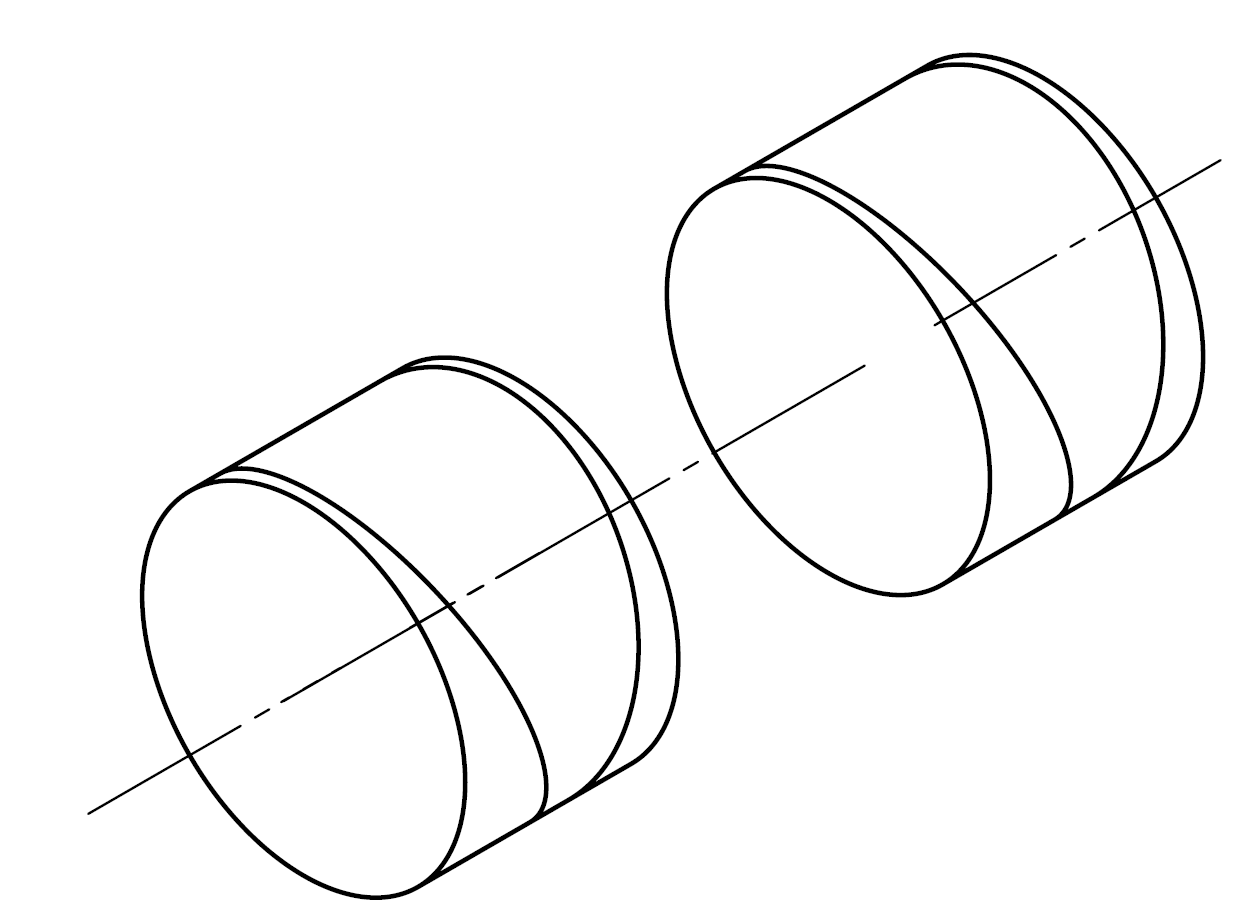
\includegraphics[width = 0.4\textwidth]{images/tripletDesignISO.png}
	\caption{2-triplet Amici prisms design \cite{KCG}}
	\centering
\end{figure}

The triplet-design seems to be appropriate for our case because it gives the best performance. However, its cost (time to design it + manufacture) is much higher than the gain we can have adding one wedge in our Amici prism. This is why we are going to design a doublet prisms ADC.\\

The system is made only by plane surfaces so that a plane front which go through the prisms should leave them as a plane front. In a collimated beam with a very narrow field of view the prisms combined thickness can be larger than the beam diameter \cite{Wynne1992}.\\
We can also use vertex with a certain radius in a converging beam. This way we can change the F\# leaving the ADC.\\
The doublet glass has to be designed in order to have a thermal expansion rate as close as possible between each glass to not break with the temperature changes. The internal reflection is also a parameter that we have to take into account because we want the ADC to transmit as much as possible light.\\

In order to design our ADC, we need to collect some information about its position in the AO bench,the dispersion of the atmosphere for our parameters, the field of view (FoV) and wavelength bandwidth it has to work in.

\subsection{Model of the atmosphere chromatic dispersion}

The atmosphere chromatic dispersion can be computed looking at the refraction index for each interesting wavelength. The following model has been implemented in order to decide which dispersion the ADC has to compensate for.

\subsubsection{Atmosphere refraction index}
First, we need to model to atsmophere dispersion (refractive index) depending on the wavelength. The simulation of the atmosphere refractive index is based on Ciddor's approach \cite{Ciddor} which is a compilation of all previous equations for the visible and near infrared. Ciddor develops a process that we can easily follow in order to model correctly the atmosphere refractive index represented by :
\begin{equation}
	n_{final} = \left(\rho_a / \rho_{axs}\right)\left(n_{axs}-1\right)+\left(\rho_\omega / \rho_{\omega s}\right)\left(n_{\omega s}-1\right)\label{eq:Ciddor_nprop}
\end{equation}
The procedure to arrive to equation~\eqref{eq:Ciddor_nprop} is described by the following sections.\\

\textbf{\underline{Point 1:} svp, $f$, $x_w$}\\
\textbf{Saturated water vapour pressure in the humid air svp}\\
\begin{equation}
	\text{svp} = \exp\left(AT^2+BT +C+\frac{D}{T}\right)\,\,\,\,\,\text{[Pa]}\label{eq:svp}
\end{equation}
With the coefficients : $A = 1.2378847\times 10^{-5}$ [K$^{-2}$], $B = -1.9121316\times 10^{-2}$ [K$^{-1}$], $C = 33.93711047$ [-], $D = -6.4341645\times 10^3$ [K])

\textbf{Enhancement factor $f$ of water vapour in the air}\\
The molar mass of dry air containing $x_\text{CO2}$ ppm of CO2~:
\begin{equation}
	M_a = \left(28.9635+12.011\times 10^{^-6}(x_\text{CO2}-400)\right)\times 10^{^-3}\,\,\,\,\,\text{[kg/mol]}\label{eq:Ma}
\end{equation}
Here we take $x_\text{CO2} = 400$ [ppm].\\
The total pressure P :
\begin{equation}
	P = P_0\left(1-\frac{\Delta T\,H}{T}\right)^{\frac{g\,M_a}{R\Delta T}}\,\,\,\,\,\text{[Pa]}\label{eq:P}
\end{equation}
With $\Delta T~=~0.0065$~[K/100 m] the vertical gradient of temperature 0.65~K for 100~m in the troposphere\cite{app:wiki_troposphere}, $H$~[m] the altitude of the site (3170~m for Karakaya), $g~=~9.80665$~[m/s$^2$] the  earth-surface gravitational acceleration and $R~=~8.314510$~[J/mol/K] the universal gas constant.
The enhancement factor :
\begin{equation}
	f = \alpha+\beta P+\gamma T^2 
\end{equation}
With $\alpha = 1.00062$~[-], $\beta  = 3.14\times 10^{-8}$~[Pa$^-1$], $\gamma = 5.6\times 10^{-7}$~[°C$^{-2}$]

\textbf{Molar fraction of water vapor in moist air $x_w$}\\
\begin{equation}
	x_w = \text{RH}\,f\frac{\text{svp}}{P} 
\end{equation}
With RH the relative humidity (RH~=~0.8 for DAG).\\

\textbf{\underline{Point 2:} n$_\text{axs}$}\\
Constants involved in the standard phase and group refractivities of dry air $k_0~=~238.0185$, $k_1~=~5792105$, $k_2~=~57.362$, $k_3~=~167917\,[\mu $m$^{-2}]$.\\
The refractive index of standard air at T=20\degree C, 101325 Pa, 0 \% humidity, 450 ppm of CO$_2$~:
\begin{equation}
	10^8 \left(n_{as}-1\right) = k_1/\left(k_0-\sigma ^2\right)+k_3/\left(k_2-\sigma ^2\right)\label{eq:naxs}
\end{equation}
With $\sigma  = 1/\lambda\,\,[\mu $m$^{^-1}]$. 
For us it is not useful to have the following equation because we are in a standard case so $n_{axs}~=~n_{as}$, but I let it in order to remember the sequence of equations :
\begin{equation}
	\left(n_{axs}-1\right) = \left(n_{as}-1\right) \left[1+0.534\times 10^{^-6}\left(x_c-450\right)\right] \label{eq:nasx}
\end{equation}
With $x_c~=~450$ [-ppm] number of ppm of CO2 (standard).\\

\textbf{\underline{Point 3:} $M_a$} see equation~\eqref{eq:Ma}.\\


\textbf{\underline{Point 4:} $Z_a$}\\
The compressibility of dry air :
\begin{equation}
	Z_\text{as} = 1-\frac{P_\text{as}}{T_\text{as}}\left[a_0+a_1\,T_\text{as}+a_2\,T_\text{as}^2+\left(b_0+b_1\,T_\text{as}\right)*x_{w\text{as}} +(c_0+c_1\,T_\text{as})*x_{w\text{as}}^2\right] +\frac{P_\text{as}^2}{T_\text{as}^2}\left(d+e*x_{w\text{as}}^2\right)\label{eq:Za}
\end{equation}
With $x_{w\text{as}}~=~0$ the molar fraction of water vapor in moist air (here we are in dry air so~0), $P_\text{as}$ [Pa] the pressure, $T_\text{as}$ [K] temperature at standard conditions and the following coefficients the compressibility factor Z~: 
\begin{multicols}{3}
$a_0~=~1.58123\times~10^{-6}\,[$K*Pa$^{-1}]$,\\
$a_1~=~-2.9331\times~10^{-8}\,[$P$a^{-1}]$,\\
$a_2~=~1.1043\times~10^{-10}\,[$(KPa)$^{-1}]$,\\
$b_0~=~5.707\times~10^{-6}\,[$K*Pa$^{-1}]$,\\
$b_1~=~-2.051\times~10^{-8}\,[$Pa$^{-1}]$,\\
$c_0~=~1.9898\times~10^{-4}\,[$K*Pa$^{-1}]$,\\
$c_1~=~-2.376\times~10^{-6}\,[$Pa$^{-1}]$,\\
$d~=~1.83\times~10^{-11}\,[$K$^2$Pa$^{-2}]$,\\
$e~=~-0.765\times~10^{-8}\,[$K$^2$Pa$^{-2}]$
\end{multicols}

\textbf{\underline{Point 5:} $Z_w$}\\
The compressibility of pure water vapour :
\begin{equation}
	Z_\text{ws} = 1-\frac{P_\text{ws}}{T_\text{ws}}\left[a_0+a_1\,T_\text{ws}+a_2\,T_\text{ws}^2+\left(b_0+b_1\,T_\text{ws}\right)*x_{w\text{ws}} +(c_0+c_1\,T_\text{ws})*x_{w\text{ws}}^2\right] +\frac{P_\text{ws}^2}{T_\text{ws}^2}\left(d+e*x_{w\text{ws}}^2\right)\label{eq:Zw}
\end{equation}
With $x_{w\text{ws}}~=~1$ the molar fraction of water vapor in moist air (here we are in moist air so~1), $P_\text{ws}~=~1333$ [Pa] the pressure, $T_\text{ws}~=~293.15$ [K] the temperature.\\

\textbf{\underline{Point 6:} $\rho_\text{axs}, \rho_\text{ws}$}\\
The density of standard dry air [kg/m$^3$]~:
\begin{equation}
	\rho_\text{axs} = \frac{P_\text{as}\,M_a}{Z_\text{as}\,R\,T_\text{as}}\left(1-x_{w\text{as}}\left(1-\frac{M_w}{M_a}\right)\right)
\end{equation}
The density of standard moist air [kg/m$^3$]~:
\begin{equation}
	\rho_\text{ws} = \frac{P_\text{ws}\,M_a}{Z_\text{ws}\,R\,T_\text{ws}}\left(1-x_{w\text{ws}}\left(1-\frac{M_w}{M_a}\right)\right)
\end{equation}
With $M_w~=~18.01528\times10^{-3}$ [kg/mol].\\

\textbf{\underline{Point 7:} $Z$}\\
The compressibility of moist air under experimental conditions~:
\begin{equation}
	Z = 1-\frac{P_\text{w}}{T_\text{w}}\left[a_0+a_1\,T_\text{w}+a_2\,T_\text{w}^2+\left(b_0+b_1\,T_\text{w}\right)*x_{w\text{w}} +(c_0+c_1\,T_\text{w})*x_{w\text{w}}^2\right] +\frac{P_\text{w}^2}{T_\text{w}^2}\left(d+e*x_{w\text{w}}^2\right)\label{eq:Zw}
\end{equation}

\textbf{\underline{Point 8:} $\rho_a$}\\
The density of the dry component of the moist air [kg/m$^3$]~:
\begin{equation}
	\rho_a = P\,Ma\frac{\left(1-x_a\right)}{Z\,R\,T_a}\label{eq:rho_a}
\end{equation}

\textbf{\underline{Point 9:} $\rho_w$}\\
The density of the dry component of the moist air [kg/m$^3$]~:
\begin{equation}
	\rho_a = P\,Ma\frac{\left(1-x_a\right)}{Z\,R\,T_a}\label{eq:rho_a}
\end{equation}

\textbf{\underline{Point 10:} $n_{final}$}\\
Constants involved in the standard phase and group refractivities of water vapour~:\\
$\omega_0 = 295.235\,[\mu $m$^{-2}],\,\,\omega_1 = 2.6422\,[\mu $m$^{-2}],\,\,\omega_2 = -0.032380\,[\mu $m$^{-4}],\,\,\omega_3 = 0.004028\,[\mu$m$^{-6}]$.\\
The refractive index of water vapour at 20°C, 1335Pa~:
\begin{equation}
	10^8 \left(n_{ws}-1\right) = 1.022\times\left(\omega_0+\omega_1\sigma^2+\omega_2\sigma^4+\omega_3\sigma^6\right)
\end{equation}

The refractive index of moist air (atmosphere)~:
\begin{equation}
	n_{final} = \left(\rho_a / \rho_{axs}\right)\left(n_{axs}-1\right)+\left(\rho_\omega / \rho_{\omega s}\right)\left(n_{\omega s}-1\right)\label{eq:Ciddor_nprop}
\end{equation}



\subsubsection{Atmosphere refraction equation}
The refraction of the atmosphere is computed with the equation \cite{Stone1996}: 
\begin{equation}
	R(\lambda,z) = \kappa\left(n(\lambda)-1\right)\left(1-\beta\right)\tan(z) - \kappa\left(n(\lambda)-1\right)\left(\beta -\frac{\left(n(\lambda)-1\right)}{2}\right)\tan^3(z)\,\,\,[\text{rad}]\label{eq:Ratm}
\end{equation}
with 
\begin{itemize}
	\item $\beta = 0.001254\left(\frac{T(K)}{273.15}\right)$ the effective height of the observatory above the surface of the earth \cite{Stone1996}
	\item $\kappa = 1$ for a spherical Earth surface \cite{Stone1996} or instrumental correction no more useful \cite{Stone2002}
\end{itemize} 
This equation~\eqref{eq:Ratm} is valid only for zenith angle $<$ 75\degree. We can even neglect the second term for zenith angles $<$ 65\degree \cite{Tendulkar}. The limit of zenith angle of our computation is set to 70\degree so the entire equation is set.\\

The model applied for the wavelength range [500, 900]~nm shows~:
\begin{figure}[H]
\centering
	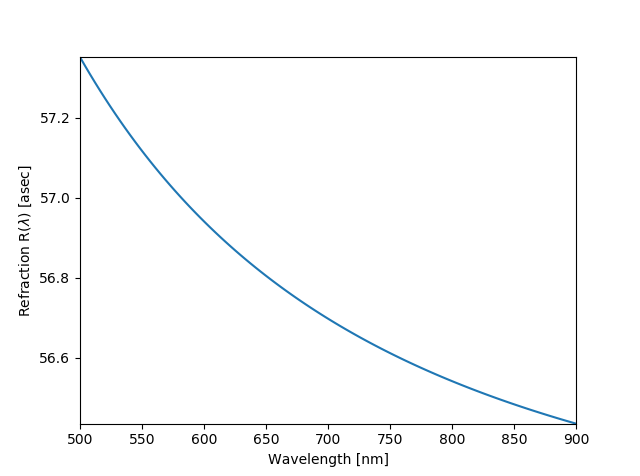
\includegraphics[width = .7\textwidth]{images/refraction_atm.png}
	\caption{Angular dispersion of the atmosphere~(appendix~\ref{app:test_Refraction_atmosphere})}\label{fig:refraction_atm}
	\centering
\end{figure}

\subsubsection{Wavelength range}
For our case, the wavelength range is set by the Nuvu camera~\cite{NuvuQE} bandwidth limits $\lambda_{min} = 500$~[nm] and $\lambda_{max} = 900$~[nm] and the maximum quantum efficiency that fixes the central wavelength to $\lambda_{cen} = 600$~[nm]. We use these 3 reference wavelengths to compute the ADC efficiency.

\subsubsection{Glasses for the ADC}
The choice of glass depends on the range of zenith angles, the wavelength interval and the cost \cite{WynneWors1986}. Most of the glass couple in the Amici conception are flint/crown pairs. \\
The glass choice is made in a data base built from Schott and Ohara catalogues. The data are taken from~\cite{RefIndexInfo} where we can download glasses properties from many different suppliers. The data are sorted to extract Sellmeier coefficients~\cite{SchottSellmeier} in order to compute the refractive index of each glass depending on the wavelength with the equation~\eqref{eq:Sellmeier}.

\begin{equation}
	n^2(\lambda) = 1+ \frac{B_1\lambda^2}{\lambda^2-C_1}+\frac{B_2\lambda^2}{\lambda^2-C_2}+\frac{B_3\lambda^2}{\lambda^2-C_3}\label{eq:Sellmeier}
\end{equation}
with $B_i$ and $C_i$ Sellmeier coefficients for $\lambda$ in $\mu$m~\cite{SchottSellmeier}.\\



\subsubsection{Beam propagation through the ADC}
In order to compute de dispersion through the ADC a geometrical and refraction set of equations have been implemented. The sequence of these equations is listed bellow. I will follow the light on the figure~\ref{fig:ADCgeometrie} to describe each step.
\begin{figure}[H]
\centering
	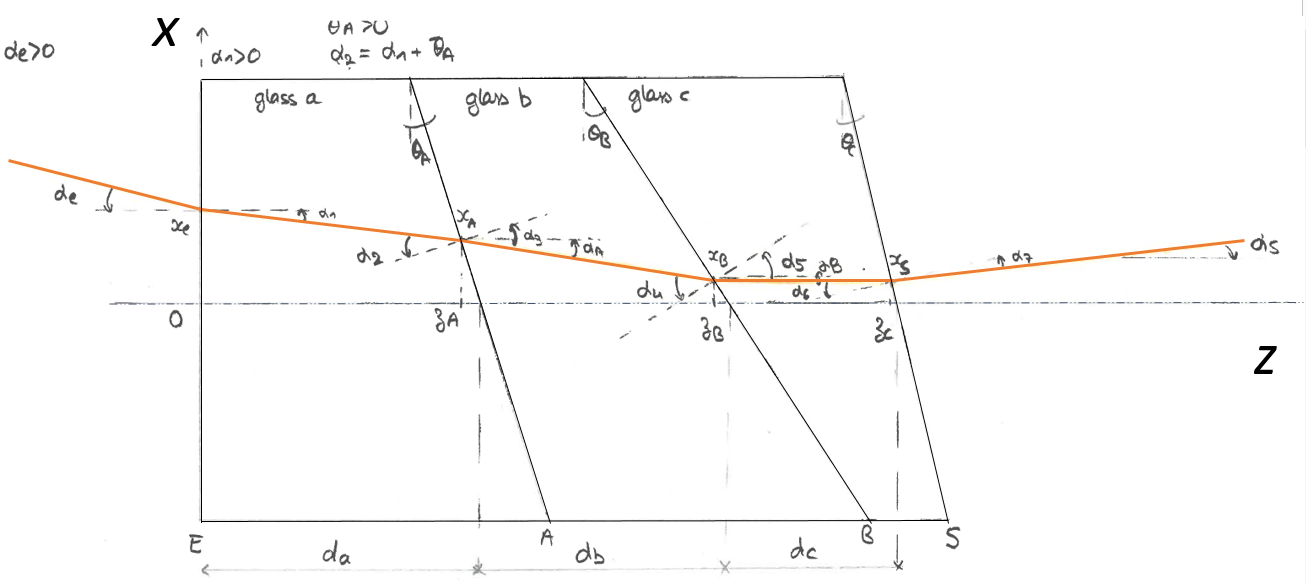
\includegraphics[width = \textwidth]{images/ADCgeometrie.png}
	\caption{Sketch of the refraction through the ADC}\label{fig:ADCgeometrie}
	\centering
\end{figure}
The refractive index of the I-th glass is $n_I(\lambda_i)$. To simplify the notation, we just write $n_I$.
We apply the sign convention described in the course material~\cite{coursOptLJT}.

The function \textit{exitAngle.py}~\ref{app:modelisationADCfunctions} computes the exit angle depending on the glass refractive index, the geometrical parameters of the prisms and the entrance angle.\\


%
%
%\paragraph*{At the entrance we have the vector}
%$\begin{bmatrix}x_E \\ z_E = 0 \\ n_0\sin\alpha_E\end{bmatrix}$
% 
%\paragraph*{At the entrance 0E, we have a refraction}
%$\begin{bmatrix}x_E \\ z_E = 0 \\ n_A\sin\alpha_1\end{bmatrix}$\\
%
%which gives :\\
%
%$\alpha_1 = \arcsin\left(\frac{n_0}{n_A}\sin\alpha_E\right) $
%
%\paragraph*{At the first interface AB, we arrive with the coordinates}
%
%$\begin{bmatrix}x_A \\ z_A \\ n_A\sin\left(\alpha_2\right)\end{bmatrix}$
%\begin{figure}[H]
%\centering
%	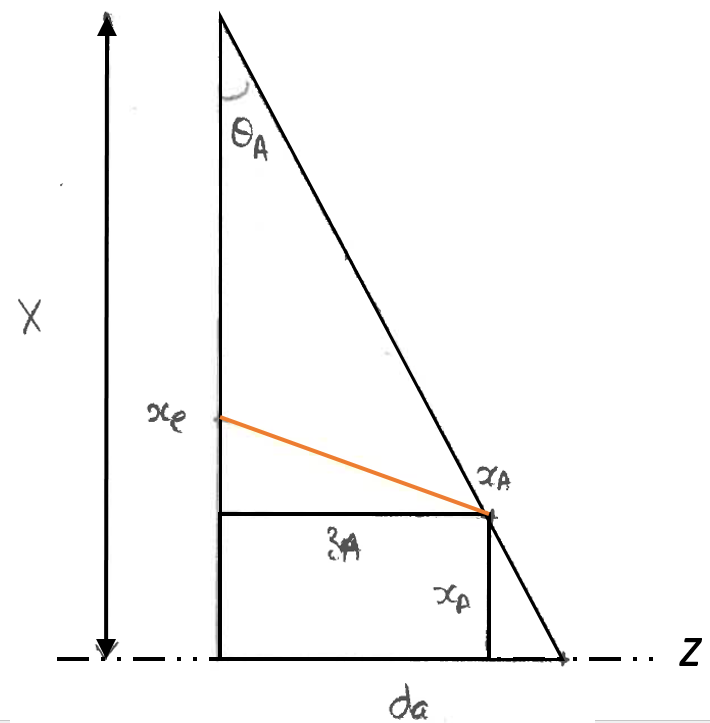
\includegraphics[width = .3\textwidth]{images/triangleGeo.png}
%	\caption{Decomposition of the parameters at an interface}\label{fig:triangle}
%	\centering
%\end{figure}
%We can determine this vector using the following equations from figure~\ref{fig:triangle} :\\
%
%$X = \frac{d_A}{\tan\theta_A}$ ; $\frac{X-x_A}{X} = \frac{z_A}{d_A}$ ; $z_A = \frac{x_E-x_A}{\tan\alpha_1}$\\
%
%Then we find :\\
%$\left \{
%   \begin{array}{r c l}
%      x_A  & = & \frac{x_E-d_A\tan\alpha_1}{1-\tan\alpha_1\tan\theta_A} \\
%      z_A   & = & \frac{x_E-x_A}{\tan\alpha1} \\
%      \alpha_2 & = & \alpha_1+\theta_A
%   \end{array}
%\right.$
%
%\paragraph*{At the interface AB, we have a refraction}
%$\begin{bmatrix}x_A \\ z_A \\ n_B\sin\alpha_3\end{bmatrix}$\\
%
%which gives :\\
%
%$\alpha_3 = \arcsin\left(\frac{n_A}{n_B}\sin\alpha_2\right) $
%
%\paragraph*{At the interface BC, we arrive with the coordinates}
%
%$\begin{bmatrix}x_B \\ z_B \\ n_B\sin\left(\alpha_4\right)\end{bmatrix}$\\
%
%We can determine this vector using the following equations from figure~\ref{fig:triangle} :\\
%
%$X = \frac{x_A}{\tan\alpha_A}$ ; $\frac{x_B}{X-Q-d_B+m} = \tan\alpha_A$ ; $m = d_A+d_B-z_B$ ; $m = x_B\tan\theta_B$ ; $Q = d_A-z_A$ ; $\alpha_A = \alpha_3+\theta_A$\\
%
%Then we find :\\
%$\left \{
%   \begin{array}{r c l}
%      x_B  & = & \frac{x_A-\tan\alpha_A\left(d_A+d_B-z_A\right)}{1-\tan\alpha_A\tan\theta_B} \\
%      z_B   & = & d_A+d_B-x_B\tan\theta_B \\
%      \alpha_4 & = & \alpha_A+\theta_B
%   \end{array}
%\right.$
%
%\paragraph*{At the interface BC, we have a refraction}
%$\begin{bmatrix}x_B \\ z_B \\ n_C\sin\alpha_5\end{bmatrix}$\\
%
%which gives :\\
%
%$\alpha_5 = \arcsin\left(\frac{n_B}{n_C}\sin\alpha_4\right) $
%
%
%\paragraph*{At the interface C0, we arrive with the coordinates}
%
%$\begin{bmatrix}x_C \\ z_C \\ n_C\sin\left(\alpha_6\right)\end{bmatrix}$\\
%
%We can determine this vector using the following equations from figure~\ref{fig:triangle} :\\
%
%$X = \frac{x_B}{\tan\alpha_B}$ ; $\frac{x_C}{X-Q-d_C+m} = \tan\alpha_B$ ; $m = d_A+d_B-z_B$ ; $m = x_C\tan\theta_C$ ; $Q = d_A+d_B-z_B$ ; $\alpha_B = \alpha_5+\theta_B$\\
%
%Then we find :\\
%$\left \{
%   \begin{array}{r c l}
%      x_C  & = & \frac{x_B-\tan\alpha_B\left(d_A+d_B+d_C-z_B\right)}{1-\tan\alpha_B\tan\theta_C} \\
%      z_B   & = & d_A+d_B+d_C-x_C\tan\theta_C \\
%      \alpha_6 & = & \alpha_B+\theta_C
%   \end{array}
%\right.$
%
%\paragraph*{At the interface C0, we have a refraction}
%$\begin{bmatrix}x_C \\ z_C \\ n_0\sin\alpha_7\end{bmatrix}$\\
%
%which gives :\\
%
%$\alpha_7 = \arcsin\left(\frac{n_C}{n_0}\sin\alpha_6\right) $\\
%
%\paragraph*{The output angle with respect to the optical axis}\
%$\alpha_S = \alpha_7-\theta_C$
%This $\alpha_S$ is the dispersion angle of the prism : $R_{prism} = \alpha_S$.
%




\subsubsection{The metric definition}
Now we have computed the dispersion of the atmosphere and the ADC. We want the smallest total dispersion after the ADC so we investigate all configurations in order to minimize it. The metric we use to calculate the efficiency of our prism combination~(appendix~\ref{app:glassChoice}) is defined by the name BDCQ (Beam Dispersion Correction Quality)~:
\begin{equation}
	\text{BDCQ}^2 = \left(\alpha_\text{Exit}\left(\lambda_{min}\right)-\alpha_\text{Exit}\left(\lambda_{av}\right)\right)^2 + \left(\alpha_\text{Exit}\left(\lambda_{max}\right)-\alpha_\text{Exit}\left(\lambda_{av}\right)\right)^2 +\\
	 \left(\alpha_\text{Exit}\left(\lambda_{av}\right)-\alpha_\text{Entry}\left(\lambda_{av}\right)\right)^2
\end{equation}


\subsubsection{Internal reflection}
In parallel of the dispersion computation, we calculate the total internal reflection of the ADC. If the refractive index of two joint glasses are too different then we will loose a lot of intensity reflected on the interface. The external faces of the ADC will be coated. The determination of the total internal reflectivity is developed below.\\
The parameters are :
\begin{itemize}
	\item $\alpha_Z = [\alpha_E;\alpha_1;\alpha_A;\alpha_B;\alpha_S]$ [rad] array of the rays angle wrt the optical axis
	\item $\alpha_I = [\alpha_1;\alpha_2;\alpha_3;\alpha_4;\alpha_5;\alpha_6;\alpha_7]$ [rad] array of the rays angles wrt the normal the vertex (refraction angle)
	\item $n = [n_0;n_A;n_B;n_C;n_0]$ medium refractive index
	\item $d = [z_A,z_B-z_A,z_C-z_B]$ [mm] distances on the optical axis between each medium change on the ray path
\end{itemize}

At the 1rst interface AB, we have~\cite{app:wiki_CoefficientsFresnel}:
\begin{equation}
	r[1] = \frac{n[3]\cos\alpha_I[2]-n[2]\cos\alpha_I[3]}{n[3]\cos\alpha_I[2]+n[2]\cos\alpha_I[3]}
\end{equation}
Taking the recursive initialization term $U(1) = r(1)$ we have for p = 2:\\
\begin{eqnarray}
	r[p] &= &\frac{n[p+1]\cos\left(\alpha_I[p]\right)-n[p]\cos\left(\alpha_I[p+1]\right)}{n[p+1]\cos\left(\alpha_I[p]\right)+n[p]\cos\left(\alpha_I[p+1]\right)}\\
	U[p] &= &\frac{U[p-1]+r[p]\exp\left(\frac{2\pi}{\lambda}\cos\left(\alpha_Z[p]\right)\,d[p-1]\right)}{1+U[p-1]\,r[p]\exp\left(\frac{2\pi}{\lambda}\cos\left(\alpha_Z[p]\right)\,d[p-1]\right)}\label{eq:Up}
\end{eqnarray}
Using equation~\eqref{eq:Up} we can calculate the reflection coefficient for $(p+1)$ number of glasses. In our case we have only 3 glasses so the total reflection (without taking external faces into account) is $U[2]$.

\subsection{ADC design optimization}
The efficiency of a combination (glass, angle) is computed by the script \textit{glassChoice.py}. The function \textit{fmin\_l\_bfgs\_b} from the optimize package in Python is used to find minimum of this constrained nonlinear multivariable function. The parameters are the geometrical coefficients for one set of glass. When the optimum is found for a combination of glass, the efficiency and internal reflection are given as outputs.\\

The global matrix is made from two for-loops that look for all glasses from the catalogues Schott and Ohara. The wavelength for which the refraction is calculated are taken from the Nuvu camera quantum efficiency curve~: $\lambda_\text{min}~=~500$ nm, $\lambda_\text{average}~=~600$ nm and $\lambda_\text{max}~=~900$ nm. The zenith angle is set to 70\degree.


\newpage
\section{DimensionnementOAPs.py}\label{app:DimensionnementOAPs}
\lstinputlisting[language=Python]{../DimensionnementOAPs.py}

\section{modelisationADCfunctions.py}\label{app:modelisationADCfunctions}
%\lstinputlisting[language=Python]{../20180611\_ADC\_design/modelisationADCfunctions.py}

\section{test\_Refraction\_atmosphere.py}\label{app:test_Refraction_atmosphere}
%\lstinputlisting[language=Python]{../20180611\_ADC\_design/test\_Refraction\_atmosphere.py}

\section{glassChoice.py}\label{app:glassChoice}
%\lstinputlisting[language=Python]{../20180611\_ADC\_design/glassChoice.py}




















